\chapter{Introducción a la Criptografía y Cuerpos Finitos}
En este capítulo voy a introducir los criptosistemas simétricos y asimétricos así como la teoría de Cuerpos Finitos, necesarios para entender el funcionamiento de los criptosistemas que se usan en las aplicaciones de mensajería.\\

\section{Objetivos de un criptosistema y posibles ataques}
Todo criptosistema se construye con la finalidad de cumplir una serie de objetivos así como de protegerse de unos ataques. A continuación voy explicar de cuales se trata.
La información de este apartado ha sido obtenida de \cite{apuntesCriptografia}.\\ 
\subsection{Objetivos}
Los objetivos que tiene que cumplir un criptosistema son los siguientes.
\begin{description}
	\item \textbf{Confidencialidad.} 
		 La información solo puede ser accesible por las entidades autorizadas. 
	\item \textbf{Integridad.} 
		La información no ha sido alterada en el envío.
	\item \textbf{Autenticidad.} 
		La información proviene de quién afirma haberla enviado.
	\item \textbf{No repudio.}  
		El emisario de una información no puede negar haber realizado tal envío.
\end{description}
\subsection{Ataques}
Para hablar de los ataques supondremos que se sigue el principio de \emph{Kerckhoffs}, el cual establece que el adversario conoce todos los detalles del criptosistema excepto la clave empleada.\\
Los posibles ataques son:
\begin{description}
		\item \textbf{Criptograma.} El adversario conoce el criptograma, es decir, el mensaje cifrado o un fragmento de este.
		\item \textbf{Mensaje Conocido.} El atacante conoce parejas mensaje/criptograma cifradas con una misma clave.
		\item \textbf{Mensaje escogido.} El atacante puede generar criptogramas para mensajes de su elección. Una vez obtenidas dichas parejas, trata de averiguar el mensaje correspondiente a un criptograma desconocido.
		\item \textbf{Mensaje escogido-adaptativo.} El atacante no solo puede generar pareas mensaje/criptograma a su elección, sino que puede hacerlo tantas veces como quiera realizando los análisis que considere oportunos.
		\item \textbf{Criptograma escogido y escogido-adaptativo.} Similar a los anteriores pero partiendo del criptograma, teniendo acceso a descifrar los criptogramas que desee, inicialmente o a lo largo del proceso. Lo que se busca en este ataque es la clave.
\end{description}

Una vez vistos los objetivos que tienen que cumplir los criptosistemas y los posibles ataques de los que pueden ser objeto, voy a explicar el uso de los criptosistemas simétricos y asimétricos en las aplicaciones de mensajería.\\

\section{Criptosistemas simétricos y asimétricos en las aplicaciones de mensajería}
Los criptosistemas simétricos y asimétricos conforman un elemento fundamental en las aplicaciones de mensajería. Criptosistemas de ambas familias se usan de manera conjunta para garantizar la confidencialidad, integridad, autenticidad y no repudio de los mensajes.\\
Los criptosistemas simétricos son utilizados para cifrar los mensajes. Esto es debido a su velocidad de cifrado, su uso reducido de recursos y su mejor manejo de grandes cantidades de datos.
Tienen el defecto de que si la clave es interceptada, el criptosistema es vulnerado y se pierde tanto la confidencialidad como la autenticidad de los mensajes. 
Para evitar esto se suele complementar con métodos seguros para el intercambio de la clave como puede ser el \emph{intercambio de claves Diffie-Hellman}.\\
Los criptosistemas asimétricos son muy utilizados para la firma y autentificación de los mensajes, garantizando de esta manera la seguridad de la aplicación y se complementan con cifrados simétricos a la hora de cifrar los mensajes para garantizar de esta forma una eficiencia mucho mayor. Ya que uno de los principales problemas que tienen es su complejidad algorítmica a la hora de cifrar y descifrar los mensajes.\\

\section{Criptosistema simétrico}
Un criptosistema simétrico es un criptosistema en el cual se utiliza una sola clave para cifrar y descifrar un mensaje o es necesario conocer la clave secreta para desencriptar un mensaje. La importancia para garantizar la seguridad de los criptosistemas simétricos reside en el secreto de la clave, mientras que el conocer el algoritmo utilizado no es tan importante como medida de seguridad. Es decir, lo importante es que el atacante no conozca la clave, mientras que conozca el algoritmo usado no lo es tanto. La información ha sido obtenida de \cite{apuntesCriptografia}.\\
Un criptosistema simétrico está formado por:
\begin{itemize}
	\item $\mathcal{M}$ el conjunto de los mensajes, elementos candidatos a ser encriptados.
	\item $\mathcal{C}$ el conjunto de los criptogramas o mensajes obtenido después del proceso de encriptar.
	\item $\mathcal{K} \subseteq \mathcal{K}_p\times\mathcal{K}_s$ el espacio de las claves, elementos que se utilizan para encriptar y desencriptar los mensajes. 
\end{itemize}
Un criptosistema simétrico viene definido por dos aplicaciones
$$E:\mathcal{K}_p\times\mathcal{M}\rightarrow\mathcal{C},$$
$$\mathcal{D}:\mathcal{K}_s\times\mathcal{C}\rightarrow\mathcal{M}.$$
tales que para cualquier clave $k_p \in \mathcal{K}_p$, existe una clave $k_s$ de manera que dato cualquier mensaje $m \in \mathcal{M}$,
$$
\mathcal{D}(k_s,E(k_p,m))=m.
$$
Fijada la clave $k_p \in \mathcal{K}_p$ y su correspondiente $k_s \in \mathcal{K}_s$ se definen las funciones de cifrado y descifrado como:\\
\begin{aligned}
	\center
	&$E_{k_p}:\mathcal{M}\rightarrow\mathcal{C},$\\
	&$E_{k_p}(m)=E(k_p,m),$
\end{aligned}
\begin{aligned}
	\center
	&$D_{k_p}:\mathcal{C}\rightarrow\mathcal{M},$\\
	&$D_{k_s}(c)=D(k_s,c),$
\end{aligned}


\subsection{Cifrados de bloque}
A continuación voy a introducir los cifrados de bloque, ya que estos son fundamentales a la hora de cifrar los mensajes en las aplicaciones de mensajería debido a su eficiencia. El cifrado de bloque más utilizado actualmente es el cifrado \textbf{Rindael AES}. La información ha sido obtenida de \cite{apuntesCriptografia}.\\
Los cifrados de bloque son criptosistemas de clave simétrica en los que la longitud de los bloques y claves es fija.\\
Este criptosistema se define
$$
	E:\mathbb{B}^K\times\mathbb{B}^N\rightarrow \mathbb{B}^N,
$$
$$
	D:\mathbb{B}^K\times\mathbb{B}^N\rightarrow \mathbb{B}^N,
$$
donde N es el tamaño del bloque y K es el tamaño de la clave.\\
Los cifrados tienen distintos modos de operación los cuales dependen solo del tamaño del bloque. Estos modos permiten garantizar la confidencialidad de los mensajes, si bien, no garantizan su integridad. La información para describir los modos la he complementado con \cite{bloquenuevo}.\\ 
Los distintos modos usados en los cifrados de bloque son:\\
\begin{itemize}
	\item \textbf{Electronic CodeBook}\\
	Modo en el cual para una clave dada, se le asigna un bloque de texto fijo cifrado por cada bloque de texto plano. Los pasos que se siguen para encriptar y desencriptar son:
	\begin{itemize}
		\item \textbf{\emph{Cifrado ECB}}
		\begin{description}
			\item Dividimos m en $m_{[1]}\dots m_{[l]}$ con $m_{[i]} \in \mathbb{B}^N$
			\item Para $i\in \{1,\dots,l\}$ hacer
			\begin{description}
				\item $c_{[i]} = E_k(m_{[i]})$
			\end{description}
			\item Devolvemos $c_{[1]}\dots c_{[l]}$
		\end{description}

		\item \textbf{\emph{Descifrado ECB}}
		\begin{description}
			\item Dividimos c en $c_{[1]}\dots c_{[l]}$ con $c_{[i]} \in \mathbb{B}^N$
			\item Para $i\in\{1,\dots,l\}$ hacer
			\begin{description}
				\item $m_{[i]} = D_k(c_{[i]})$
			\end{description}
			\item Devolvemos $m_{[1]}\dots m_{[l]}$
		\end{description}
	\end{itemize}
%\newpage
		\begin{figure}[htb]
			\centering
			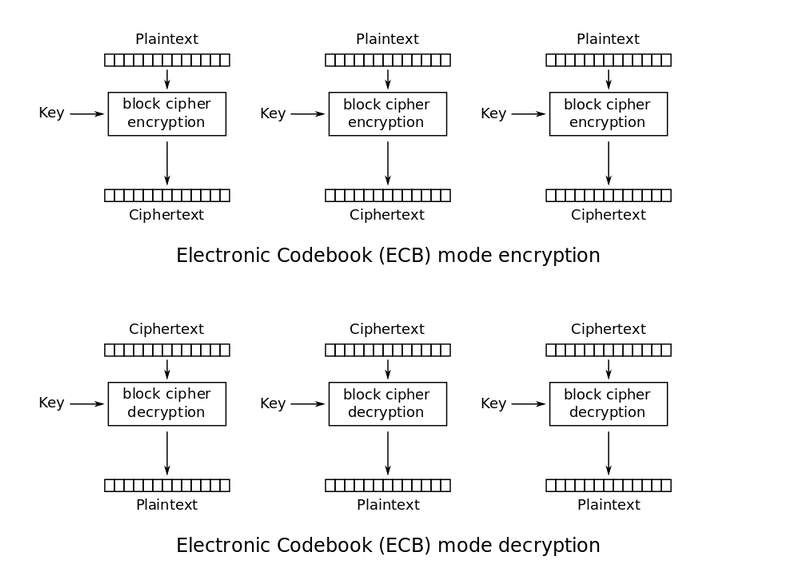
\includegraphics[scale=0.4]{imagenes/ecb.png} 
			\caption{Esquema del cifrado y descifrado del modo ECB \cite{cifradobloque}.}
			\label{esquemaecb}
		\end{figure}
		
	\item \textbf{Cipher-Block Chaining}\\
	En este modo se combina los bloques de texto plano con los bloques de texto cifrados anteriormente. Para cifrar el primer bloque será necesario un bloque inicial, $c_{[0]}$, el cual no tiene necesariamente que ser secreto. Los pasos seguidos para encriptar y desencriptar son:
	\begin{itemize}
		\item \textbf{\emph{Cifrado CBC}}
		\begin{description}
			\item $c_{[0]} \in \mathbb{B}^*$
			\item Dividimos m en $m_{[1]}\dots m_{[l]}$ con $m_{[i]} \in \mathbb{B}^N$
			\item Para $i\in\{1,\dots,l\}$ hacer
			\begin{description}
				\item $c_{[i]} = E_k(m_{[i]}\oplus c_{[i-1]})$
			\end{description}
			\item Devolvemos $c_{[1]}\dots c_{[l]}$
		\end{description}

		\item \textbf{\emph{Descifrado CBC}}
		\begin{description}
			\item Dividimos c en $c_{[0]}\dots c_{[l]}$ con $c_{[i]} \in \mathbb{B}^N$
			\item Para $i\in\{1,\dots,l\}$ hacer
			\begin{description}
				\item $m_{[i]} = D_k(c_{[i]})\oplus c_{[i]}$
			\end{description}
			\item Devolvemos $m_{[1]}\dots m_{[{l}]}$
		\end{description}
	\end{itemize}
\newpage
		\begin{figure}[htb]
			\centering
			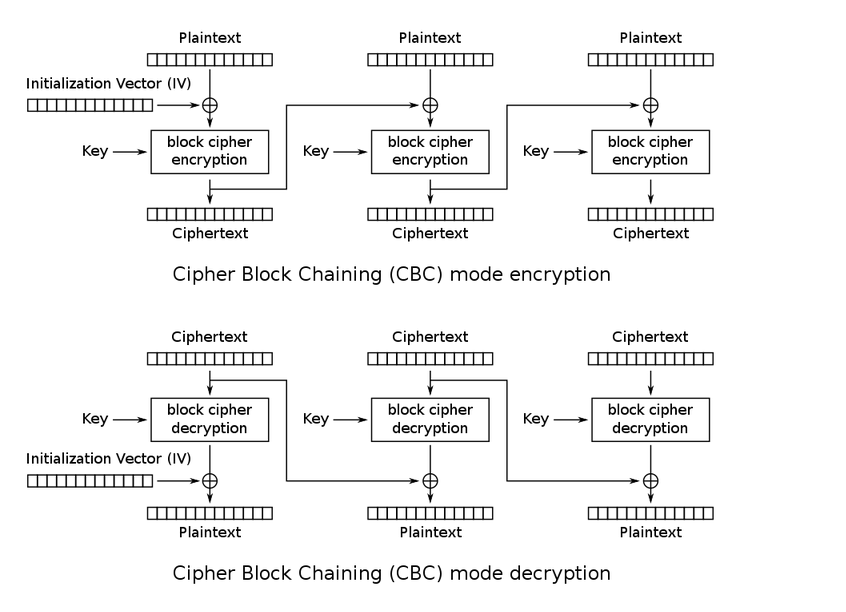
\includegraphics[scale=0.4]{imagenes/cbc.png} 
			\caption{Esquema del cifrado y descifrado del modo CBC \cite{cifradobloque}.}
			\label{esquemacbc}
		\end{figure}

	\item \textbf{Cipher FeedBack}\\
	Modo en el cual se combina cada bloque de texto plano del mensaje consigo mismo encriptado, los pasos que se siguen son:
	\begin{itemize}
		\item \textbf{\emph{Cifrado CFB}}
		\begin{description}
			\item $x_{[0]} \in \mathbb{B}^r$
			\item Dividimos m en $m_{[1]}\dots m_{[l]}$ con $m_{[i]} \in \mathbb{B}^N$
			\item Para $i\in\{1,\dots,l\}$ hacer
			\begin{description}
				\item $c_{[i]} = m_{[i]}\oplus msb_r(E_k(x_{[i]}))$
				\item $x_{[i+1]} = lsb_{N-r}(x_i)||c_{[i]$
			\end{description}
			\item Devolvemos $c_{[1]}\dots c_{[l]}$
		\end{description}

		\item \textbf{\emph{Descifrado CFB}}
		\begin{description}
			\item Dividimos c en $c_{[1]}\dots c_{[l]}$ con $c_{[i]} \in \mathbb{B}^r$
			\item Para $i\in\{1,\dots,l\}$ hacer
			\begin{description}
				\item $m_{[i]} = c_{[i]}\oplus msb_r(E_k(x_{[i]}))$
				\item $x_{[i+1]} = lsb_{N-r}(x_i)||c_{[i]$
			\end{description}
			\item Devolvemos $m_{[1]}\dots m_{[l]}$
		\end{description}
	\end{itemize}

%\newpage
		\begin{figure}[htb]
			\centering
			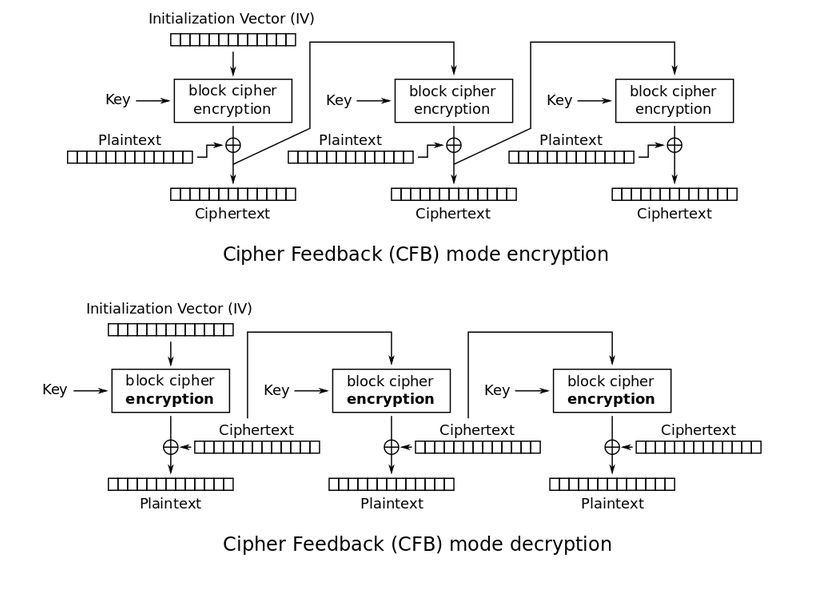
\includegraphics[scale=0.4]{imagenes/cfb.png} 
			\caption{Esquema del cifrado y descifrado del modo CFB \cite{cifradobloque}.}
			\label{esquemacfb}
		\end{figure}

\newpage
	\item \textbf{Output FeedBack}\\
	Modo en el cual se parte de un bloque inicial $x_{[0]}$ único y secreto. En cada iteración se encripta este y se combina con un bloque del mensaje sin cifrar de manera recursiva. Los pasos seguidos para encriptar y desencriptar son:
	\begin{itemize}
		\item \textbf{\emph{Cifrado OFB}}
		\begin{description}
			\item $x_{[0]} \in \mathbb{B}^N$
			\item Dividimos m en $m_{[1]}\dots m_{[l]}$ con $m_{[i]} \in \mathbb{B}^N$
			\item Para $i\in\{1,\dots,l\}$ hacer
			\begin{description}
				\item $x_{[i]} = E_k(x_{[i-1]})$
				\item $c_{[i]} = m_{[i]}\oplus x_{[i]}$
			\end{description}
			\item Devolvemos $c_{[1]}\dots c_{[l]}$
		\end{description}

		\item \textbf{\emph{Descifrado OFB}}
		\begin{description}
			\item Dividimos c en $c_{[1]}\dots c_{[l]}$ con $c_{[i]} \in \mathbb{B}^N$
			\item Para $i\in\{1,\dots,l\}$ hacer
			\begin{description}
				\item $x_{[i]} = E_k(x_{[i-1]})$
				\item $m_{[i]} = c_{[i]}\oplus x_{[i]}$
			\end{description}
			\item Devolvemos $m_{[1]}\dots m_{[l]}$
		\end{description}
	\end{itemize}
		\begin{figure}[htb]
			\centering
			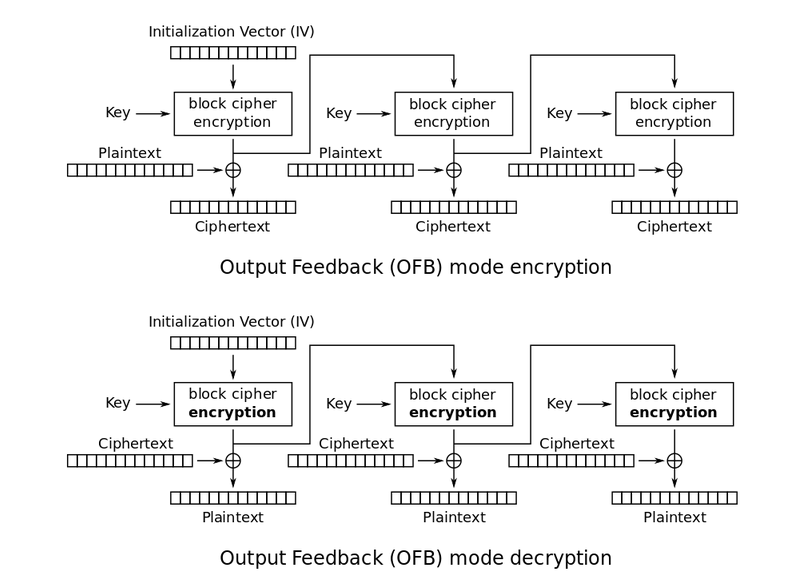
\includegraphics[scale=0.4]{imagenes/ofb.png} 
			\caption{Esquema del cifrado y descifrado del modo OFB \cite{cifradobloque}.}
			\label{esquemaofb}
		\end{figure}

\newpage

	\item \textbf{Galois Counter Mode (GCM)}\\
	Modo en el cual se usa un función hash universal sobre un cuerpo de Galois binario que provee de una autentica encriptación. La información de este modo ha sido obtenida de \cite{gcm}.
		Para cifrar en este modo partimos de una entrada con 4 elementos. 
		\begin{itemize}
			\item \emph{K} que es una clave secreta.
			\item \emph{IV} vector inicial que puede tener un número de bits entre 1 y $2^{64}$.
			\item \emph{P} texto plano que puede tener un número de bits contenido entre 0 y $2^{39}-256$.
			\item \emph{AAD} datos de autentificación adicionales, \emph{Additional Authenticated Data}, que puede tener un tamaño entre 0 y $2^{64}$ bits.
		\end{itemize}
		Y en la salida devuelve $C$ que es el texto encriptado y una autentificación $T$.\\
		Una vez visto la entrada y la salida, el algoritmo de cifrado y descifrado quedarían como sigue.
		\newpage
	\begin{itemize}
		\item \textbf{\emph{Cifrado GCM}}
		\begin{description}
			\item $H=E(0^{128})$
			\item Si $len(IV)=96$
			\begin{description}
				\item $Y_0=IV||0^{31}1$
			\end{description}
			\item si no
			\begin{description}
				\item $Y_0=GHASH(H,\{\},IV)$
			\end{description}
			\item Para $i\in\{1,\dots,n-1\}$ hacer
			\begin{description}
				\item $Y_i=incr(Y_{i-1})$
				\item $C_i=P_i\oplus E(Y_i)$
			\end{description}
			\item $Y_n=incr(Y_{n-1})$
			\item $C_n=P_n\oplus MSB_u(E(Y_n))$
			\item $T=MSB_t(GHASH(H,A,C)\oplus E(Y_0))$
		\end{description}
		Donde $C=C_1,\dots, C_n$, $A=A_1,\dots,A_m$, $incr(F||I)= F||(I+1\mod 2^{32})$ y la función $GHASH(H,A,C)$ equivale a calcular $X_{m+n+1}$. $X_i$ es una variable que se calcula como  
		
		\begin{equation}
		  X_i =
			\begin{cases}
				0 & \text{si } i= 0, \\
				(X_{i-1}\oplus A_i)\cdot H & \text{si } i\in\{1,\dots,m-1\}, \\
				(X_{m-1}\oplus(A_m||0^{128-v}))\cdot H & \text{si } i= m, \\
				(X_{i-1}\oplus C_i)\cdot H & \text{si } i\in\{m+1,\dots,m+n-1\}, \\
				(X_{m+n-1}\oplus(C_m||0^{128-u}))\cdot H & \text{si } i= m+n, \\
				(X_{m+n}\oplus(len(A)||len(C)))\cdot H & \text{si } i=m+n+1.
			\end{cases}       
			\notag
		\end{equation}

		\item \textbf{\emph{Descifrado GCM}}
		\begin{description}
			\item $H=E(0^{128})$
			\item Si $len(IV)=96$
			\begin{description}
				\item $Y_0=IV||0^{31}1$
			\end{description}
			\item si no
			\begin{description}
				\item $Y_0=GHASH(H,\{\},IV)$
			\end{description}
			\item $T^{'}=MSB_t(GHASH(H,A,C)\oplus(Y_0))$
			\item Para $i\in\{1,\dots,n-1\}$ hacer
			\begin{description}
				\item $Y_i=incr(Y_{i-1})$
				\item $P_i=C_i\oplus E(Y_i)$
			\end{description}
			\item $Y_n=incr(Y_{n-1})$
			\item $P_n=C_n\oplus MSB_u(E(Y_n))$
			\item $T=MSB_t(GHASH(H,A,C)\oplus E(Y_0))$
		\end{description}
		Si T y T' coinciden entonces se devuelve el texto descifrado. Si no coinciden, entonces el texto no se devuelve ya que eso implicaría que el mensaje ha sido manipulado.
	\end{itemize}
		\begin{figure}[htb]
			\centering
			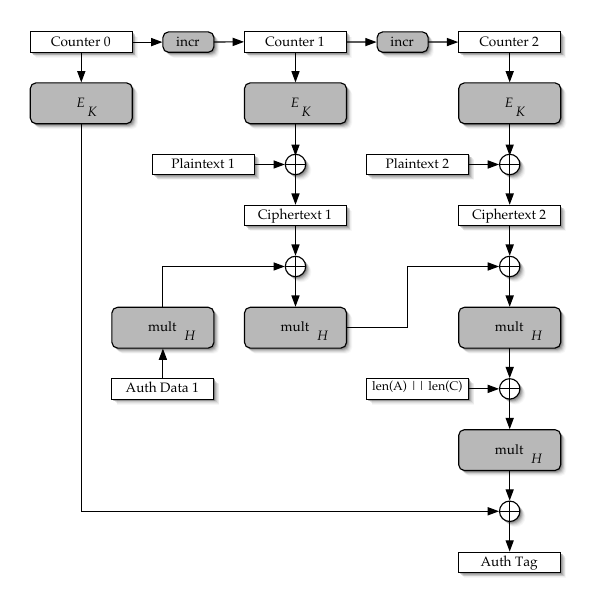
\includegraphics[scale=0.4]{imagenes/cgc.png} 
			\caption{Esquema del cifrado y descifrado del modo GCM \cite{gcm}.}
			\label{esquemaofb}
		\end{figure}
\end{itemize}
%\newpage
Como podemos ver, el más sencillo es ECB ya que lo único que hace es fragmentar el mensaje en bloques y encriptar individualmente cada bloque. En CBC, CFB, OFB y GCM se parte de un bloque inicial y se generan bloques nuevos de manera recursiva operando con ellos de manera distinta en función de cada modo.\\ 
En CBC se realiza la operación $\oplus$ de cada bloque generado encriptándose el bloque cifrado previo a esta con un bloque del mensaje, los nuevos bloques son los resultados de la operación anterior.\\
En CFB se coge el bit menos significativo resultante de encriptar el bloque generado previo y se hace la operación $\oplus$ con cada bloque del mensaje. Para generar un nuevo bloque se combina el mensaje cifrado previo con el bit menos significativo del conjunto de bits $N-r$ del bloque generado anterior con la operación $||$.\\
En OFB se realiza la operación $\oplus$ de el resultado de encriptar el bloque generado previo con un bloque del mensaje.\\
Y en GCM lo que se hace es fragmentar el mensaje y operar con los fragmentos de manera recursiva usando una función hash universal (\emph{GHASH}) con el primer bloque, además se realiza una operación paralela que se almacena en $T$ para certificar la integridad del mensaje.\\
Actualmente el más utilizado en las aplicaciones de mensajería es el modo CBC. Esto es debido a que es relativamente fácil de implementar y además permite encriptar en paralelo. Si bien, está empezando a utilizarse el modo GCM ya que implementado en hardware permite unas velocidades muy altas de encriptado llegando incluso a poder encriptar 10 GB por segundo. Un ejemplo de ello es la aplicación Line, que en su segunda versión incorpora este modo. 

\section{Criptosistema asimétrico}
Un criptosistema asimétrico es un criptosistema en el cual se utilizan dos claves, una para cifrar el mensaje y otra para descifrarlo. La clave para cifrar es la que se conoce como \emph{clave pública}, mientras que la que se utiliza para descifrar es la \emph{clave privada}. Estos criptosistemas surgieron para paliar la debilidad de los criptosistemas simétricos, que es que la clave que cifra y descifra se tiene que compartir, pudiendo esta ser interceptada.  
La seguridad de estos criptosistemas reside en que no se conozca la clave privada. La información ha sido obtenida de \cite{angelRiosMateos}.\\
Un criptosistema asimétrico está formado por:
\begin{itemize}
	\item $\mathcal{M}$ es el conjunto de los mensajes.
	\item $\mathcal{C}$ es el conjunto de los criptogramas.
	\item Una función $P:\mathcal{K}' \rightarrow \mathcal{K}$, que nos permitirá generar la clave pública. De manera que para cualquier clave privada $k' \in \mathcal{K}'$ obtenemos la clave pública como $P(k')=k$ 
\end{itemize}
Un criptosistema asimétrico viene definido por dos aplicaciones:
$$E:\mathcal{K}\times\mathcal{M}\rightarrow\mathcal{C},$$
$$\mathcal{D}:\mathcal{K}'\times\mathcal{C}\rightarrow\mathcal{M},$$
y se definen las funciones de cifrado y descifrado como:\\
\begin{aligned}
	\center
	&$E_{k}:\mathcal{M}\rightarrow\mathcal{C},$\\
	&$E_{k}(m)=E(k,m),$
\end{aligned}
\begin{aligned}
	\center
	&$D_{k^{'}}:\mathcal{C}\rightarrow\mathcal{M},$\\
	&$D_{k'}(c)=D(k',c).$
\end{aligned}

Para que un criptosistema asimétrico sea seguro tenemos que garantizar:
\begin{itemize}
	\item $P$ es una función de dirección única, es decir, que dado un elemento de su imagen no se puede calcular su imagen inversa fácilmente.
	\item Para la mayoría de los $k \in \mathcal{K}$, la aplicación $E_k$ es de dirección única.
	\item $\mathcal{D}_{k'}$ se puede calcular en un periodo corto de tiempo si se conoce $k'$ y es imposible o el periodo es muy largo en caso de solo conocerse $k$.
\end{itemize}

\section{El cuerpo de Galois $\operatorname{GF}(2^n)$}
Tanto para explicar el funcionamiento de las rondas de AES como para desarrollar la teoría de Curvas Elípticas en $\operatorname{GF}(2^n)$ es necesario introducir el cuerpo $\operatorname{GF}(2^n)$. El cual debido a las propiedades que tiene es muy utilizado en criptografía.\\
Sea $\mathbb{Z}_2[x]$ el conjunto de polinomios con coeficientes en $\mathbb{Z}_2$, es decir, el conjunto de polinomios cuyos coeficientes solo valen 0 ó 1. Así los polinomios pueden ser representados por una cadena de bits.
 Un ejemplo sería el polinomio $f(x)=x^4+x^3+x+1$ que quedaría representado como 11011. 
Además si lo sumamos con otro polinomio como puede ser $g(x)=x^2+x+1$, tenemos que $f(x)+g(x)=x^4+x^3+x^2$, que equivale a hacer la operación XOR entre 11011 y 00111, por lo que a nivel computacional, es muy fácil implementar estas operaciones.\\
Podemos definir el cuerpo $\operatorname{GF}(2^n)$ como $\mathbb{Z}_2[x]/(a(x))$, con $a(x)$ un polinomio irreducible en $\mathbb{Z}/(a(x))$. Tenemos que la existencia del inverso de cualquier polinomio no nulo está asegurada por el algoritmo Extendido de Euclídes.\\ 
Principalmente se trabaja con $\operatorname{GF}(2^n)$ debido a que la implementación de las operaciones de este es más sencilla que la implementación en las que se utilizan otros cuerpos. Ya que como hemos visto, es muy fácil implementar las operaciones. Por lo que teniendo el mismo orden de complejidad, se multiplica la velocidad permitiendo obtener sistemas con mejores prestaciones.\\
A continuación presentaré el cuerpo $\operatorname{GF}(2^8)$ ya que será necesario para entender adecuadamente las operaciones utilizadas en AES. La información ha sido obtenida de \cite{criptografia} y \cite{dem1}.\\
Tenemos que $\operatorname{GF}(2^8)=\mathbb{F}_{256}$ por lo que por comodidad trabajaremos con este último.\\
Por definición tenemos que para $p$ número primo y $n$ se define el cuerpo $\mathbb{F}_{p^n}$ al único cuerpo existente con $p^n$ elementos. En particular para trabajar con $\mathbb{F}_{256}$ tomamos $p=2$ y $n=8$.\\
Para construir $\mathbb{F}_{256}$ necesitamos un polinomio de grado 8, con coeficientes en $\mathbb{Z}_2$ y que sea irreducible. En total hay 30 polinomios con esas características donde algunos de ellos son 
$x^8+x^4+x^3+x+1$, $\:x^8+x^4+x^3+x^2+1$, $x^8+x^5+x^3+x+1$, $x^8+x^5+x^3+x^2+1$, $x^8+x^5+x^4+x^3+1$, $x^8+x^5+x^4+x^3+x^2+x+1$ y $x^8+x^6+x^3+x^2+1$.\\ 
Cabe a destacar que cualquiera de los polinomios serviría para definir $\mathbb{F}_{256}$ y además no habría ninguna diferencia en la seguridad en los criptosistemas que lo utilicen. 
Para AES se tomó el polinomio $x^8+x^4+x^3+x+1$, por lo que a partir de ahora trabajaremos con $\mathbb{Z}_{2_{x^8+x^4+x^3+x+1}}[x]$.\\
Los elementos que conformarán al cuerpo serán clases de equivalencia de polinomios  de grado menor que 8. Cada elemento podrá ser representado de tres formas distintas además de la forma polinomial, como número binario, número hexadecimal y número decimal. Por ejemplo el polinomio $x^5+x+1$ quedaría representado como $00100011$ de manera decimal, $23$ en hexadecimal y $35$ en decimal.\\
Al ser $\mathbb{F}_{256}$ un cuerpo tenemos que tiene dos operaciones, la operación suma que representaremos como $+$ y la operación producto que representaremos como $\cdot$.\\
La operación $+$ equivale a la suma en $\mathbb{Z}_2$ y usando la notación en binario, tendríamos que equivaldría con la operación XOR como ya he mencionado anteriormente. El opuesto para la suma de un elemento equivalente a sí mismo por lo que no habría diferencia entre sumar por un número o por su apuesto, luego tendríamos que la suma es la misma operación que la resta.\\
La operación $\cdot$  es mucho más compleja ya que en principio habría que realizar la operación en notación polinomial y luego calcular el resto de dividir por $x^8+x^4+x^3+x+1$. Para calcular el inverso tendríamos que utilizar el algoritmo extendido de Euclídes. Ambos algoritmos tienen una complejidad algorítmica importante, pero se puede reducir. A continuación desarrollaré unos resultados de cuerpos finitos que nos permitirá obtener unos métodos que reducirán mucho esa complejidad.\\
\begin{definicion}
	Sea $K=\mathbb{F}_q$ un cuerpo finito $(q=p^n)$. Un elemento primitivo de $K$ es un elemento $\alpha$ que tiene $q-1$ potencias distintas.
\end{definicion}

\begin{teorema}
	(Teorema Fundamental de los Grupos Abelianos) Todo grupo abeliano finito $G$ es isomorfo a un producto directo de grupo cíclicos de la forma
	$$
		\mathbb{Z}_{p^{\alpha_1}_1}\times \dots \times \mathbb{Z}_{p^{\alpha_n}_n},
	$$
	donde los $p_i$ son primos no necesariamente diferentes.
\end{teorema}

\begin{teorema}
		Si $G$ es un subgrupo finito de $F^*$, el grupo multiplicativo de elementos no nulos de un cuerpo $F$, entonces $G$ es cíclico.
\end{teorema}\vspace*{-7mm}
\begin{proof}
		Sea $G$ un subgrupo finito de $F^*$ de orden $n$. Por el Teorema Fundamental de Grupos Abelianos tenemos,
		$$
			G \cong \mathbb{Z}_{p^{e_1}_1}\times \dots \times \mathbb{Z}_{p^{e_k}_k},
		$$
		donde $n = p^{e_1}_1 \dots p^{e_k}_k$ y los $p_1, \dots, p_k$ son primos no necesariamente distintos. Sea $m$ el mínimo común múltiplo de $p^{e_1}_1 \dots p^{e_k}_k$. Entonces $G$ contiene un elemento de orden $m$. Como todo $\alpha$ en $G$ satisface $x^r-1$ para algún $r$ que divide a $m$, $\alpha$ debe también ser raíz de $x^m-1$. Como $x^m-1$ tienen a lo más $m$ raíces en $F$, $n\leq m$. Por otra parte, sabemos que $m\leq |G|$, por lo tanto, $m=n$. Luego $G$ contiene un elemento de orden $n$ y tiene que ser cíclico.\qedhere
\end{proof}

\begin{corolario}
		El grupo multiplicativo de todos los elementos no nulos de un cuerpo finito es cíclico.
\end{corolario}

Por lo que si $\alpha$ es un elemento primitivo de $\mathbb{F}_q$, los $q-1$ elementos de la forma\\
$$
	\alpha^0=1,\;\; \alpha^1=\alpha,\;\dots\; ,\alpha^{q-2}
$$
serán todos independientes, es decir, distintos y no nulos. Por tanto serán todos los elementos no nulos de $\mathbb{F}_q$. Además, se verifica que $\alpha^{q-1}=\alpha^0$ por lo que para cualquier $n \in \mathbb{Z}$ se cumple que $\alpha^n=\alpha^{n\mod q-1}$.\\

\begin{teorema}
	Todo cuerpo finito tiene al menos un elemento primitivo.
\end{teorema}
Salvo para $q=2$, el número de elementos primitivos de $\mathbb{F}_q$ es $\phi(q-1)$. Para el caso $q=13$ se tiene que $\phi(12)=\phi(2^2\cdot 3)=2\cdot2=4$, luego $\mathbb{Z}_{13}$ tiene 4 elementos primitivos que son 2, 6, 7 y 11. En $\mathbb{F}_{256}$ tenemos que hay $\phi(256)=128$ elementos primitivos.

Ahora para multiplicar dos elementos pertenecientes a $\mathbb{Z}_{13}$ podemos usar su logaritmo en base 2, el exponente que hay que elevar 2 para obtener el número, sumar los logaritmos y reducirlos base 13 y elevar 2 al resultado. Un ejemplo sería:
$$
	10\cdot12=2^{10}\cdot2^{6}=2^{16}=2^3=8.
$$
Para calcular el inverso sería:
$$
	12^{-1}=(2^6)^{-1}=2^{12-6}=2^6=12.
$$
Esta es la idea que nos permite optimizar las multiplicaciones y los cálculos de inversos en $\mathbb{F}_{256}$. Para ello elegimos un elemento primitivo que nos servirá de generador, en este caso nosotros utilizaremos el más pequeño, que es $[x+1]$ en notación polinomial, 00000011 en binario, 03 en hexadecimal y 3 en binario. Por comodidad trabajaremos en hexadecimal. 

\begin{table}[!htb]
    %\begin{adjustwidth}{-.8in}{-.8in}  
\resizebox{\textwidth}{!}{%
\begin{tabular}{|l|l|l|l|l|l|l|l|l|l|l|l|l|l|l|l|l|}
\hline
\multicolumn{1}{|r|}{} & 0  & 1  & 2  & 3  & 4  & 5  & 6  & 7  & 8  & 9  & A  & B  & C  & D  & E  & F  \\ \hline
0                      & 01 & 03 & 05 & 0F & 11 & 33 & 55 & FF & 1A & 2E & 72 & 96 & A1 & F8 & 13 & 35 \\ \hline
1                      & 5F & E1 & 38 & 48 & D8 & 73 & 95 & A4 & F7 & 02 & 06 & 0A & 1E & 22 & 66 & AA \\ \hline
2                      & E5 & 34 & 5C & E4 & 37 & 59 & EB & 26 & 6A & BE & D9 & 70 & 90 & AB & E6 & 31 \\ \hline
3                      & 53 & F5 & 04 & 0C & 14 & 3C & 44 & CC & 4F & D1 & 68 & B8 & D3 & 6E & B2 & CD \\ \hline
4                      & 4C & D4 & 67 & A9 & E0 & 3B & 4D & D7 & 62 & A6 & F1 & 08 & 18 & 28 & 78 & 88 \\ \hline
5                      & 83 & 9E & B9 & D0 & 6B & BD & DC & 7F & 81 & 98 & B3 & CE & 49 & DB & 76 & 9A \\ \hline
6                      & B5 & C4 & 57 & F9 & 10 & 30 & 50 & F0 & 0B & 1D & 27 & 69 & BB & D6 & 61 & A3 \\ \hline
7                      & FE & 19 & 2B & 7D & 87 & 92 & AD & EC & 2F & 71 & 93 & AE & E9 & 20 & 60 & A0 \\ \hline
8                      & FB & 16 & 3A & 4E & D2 & 6D & B7 & C2 & 5D & E7 & 32 & 56 & FA & 15 & 3F & 41 \\ \hline
9                      & C3 & 5E & E2 & 3D & 47 & C9 & 40 & C0 & 5B & ED & 2C & 74 & 9C & BF & DA & 75 \\ \hline
A                      & 9F & BA & D5 & 64 & AC & EF & 2A & 7E & 82 & 9D & BC & DF & 7A & 8E & 89 & 80 \\ \hline
B                      & 9B & B6 & C1 & 58 & E8 & 23 & 65 & AF & EA & 25 & 6F & B1 & C8 & 43 & C5 & 54 \\ \hline
C                      & FC & 1F & 21 & 63 & A5 & F4 & 07 & 09 & 1B & 2D & 77 & 99 & B0 & CB & 46 & CA \\ \hline
D                      & 45 & CF & 4A & DE & 79 & 8B & 86 & 91 & A8 & E3 & 3E & 42 & C6 & 51 & F3 & 0E \\ \hline
E                      & 12 & 36 & 5A & EE & 29 & 7B & 8D & 8C & 8F & 8A & 85 & 94 & A7 & F2 & 0D & 17 \\ \hline
F                      & 39 & 4B & DD & 7C & 84 & 97 & A2 & FD & 1C & 24 & 6C & B4 & C7 & 52 & F6 & 01 \\ \hline
\end{tabular}}
	\label{antilogaritmos}
	%\end{adjustwidth}
\caption{Tabla de los antilogaritmos de $[x+1]$}
\end{table}
Por ejemplo para calcular el resultado de $[x+1]^{125}=(03)^{125}$ lo que hacemos es escribir 125 en hexadecimal que es 7D. A continuación miramos en la tabla, la fila 7 y la columna D que nos da 20 luego tendríamos que $(03)^{125}=20$. Pasándolo a forma polinomial tenemos que $[x+1]^{125}=x^5$.\\
Para construir la tabla es mejor usar la forma binaria.\\

A continuación vamos a construir la tabla inversa de la anterior, esta nos permitirá calcular dado un $z \in \mathbb{F}_{256}$ con $z \neq 0$ el valor de $y$ que verifica $[x+1]^y=z$ que denominaremos $\log_{x+1}(z)$.
\begin{table}[!htb]
    %\begin{adjustwidth}{-.8in}{-.8in}  
\resizebox{\textwidth}{!}{%
\begin{tabular}{|l|l|l|l|l|l|l|l|l|l|l|l|l|l|l|l|l|}
\hline
  & 0  & 1  & 2  & 3  & 4  & 5  & 6  & 7  & 8  & 9  & A  & B  & C  & D  & E  & F  \\ \hline
0 &    & 00 & 19 & 01 & 32 & 02 & 1A & C6 & 4B & C7 & 1B & 68 & 33 & EE & DF & 03 \\ \hline
1 & 64 & 04 & E0 & 0E & 34 & 8D & 81 & EF & 4C & 71 & 08 & C8 & F8 & 69 & 1C & C1 \\ \hline
2 & 7D & C2 & 1D & B5 & F9 & B9 & 27 & 6A & 4D & E4 & A6 & 72 & 9A & C9 & 09 & 78 \\ \hline
3 & 65 & 2F & 8A & 05 & 21 & 0F & E1 & 24 & 12 & F0 & 82 & 45 & 35 & 93 & DA & 6E \\ \hline
4 & 96 & 8F & DB & BD & 36 & D0 & CE & 94 & 13 & 5C & D2 & F1 & 40 & 46 & 83 & 38 \\ \hline
5 & 66 & DD & FD & 30 & BF & 06 & 8B & 62 & B3 & 25 & E2 & 98 & 22 & 88 & 91 & 10 \\ \hline
6 & 7E & 6E & 48 & C3 & A3 & B6 & 1E & 42 & 3A & 6B & 28 & 54 & FA & 85 & 3D & BA \\ \hline
7 & 2B & 79 & 0A & 15 & 9B & 9F & 5E & CA & 4E & D4 & AC & E5 & F3 & 73 & A7 & 57 \\ \hline
8 & AF & 58 & A8 & 50 & F4 & EA & D6 & 74 & 4F & AE & E9 & D5 & E7 & E6 & AD & E8 \\ \hline
9 & 2C & D7 & 75 & 7A & EB & 16 & 0B & F5 & 59 & CB & 5F & B0 & 9C & A9 & 51 & A0 \\ \hline
A & 7F & 0C & F6 & 6F & 17 & 74 & 49 & EC & D8 & 43 & 1F & 2D & A4 & 76 & 7B & B7 \\ \hline
B & CC & BB & 3E & 5A & FB & 60 & B1 & 86 & 3B & 52 & A1 & BC & AA & 55 & 29 & 9D \\ \hline
C & 97 & B2 & 87 & 90 & 61 & BE & DC & FC & B5 & 95 & CF & CD & 37 & 3F & 5B & D1 \\ \hline
D & 53 & 39 & 84 & 3C & 41 & A2 & 6D & 47 & 14 & 2A & 9E & 5D & 56 & F2 & D3 & AB \\ \hline
E & 44 & 11 & 92 & D9 & 23 & 20 & 2D & 89 & B4 & 7C & B8 & 26 & 77 & 99 & E3 & A5 \\ \hline
F & 67 & 48 & ED & DE & C5 & 31 & FE & 18 & 0D & 63 & 8C & 80 & C0 & F7 & 70 & 07 \\ \hline
\end{tabular}}
	\label{potenciasinversas}
    %\end{adjustwidth}
\caption{Tabla de los logaritmos de $[x+1]$}
\end{table}
\newpage
A partir de estas dos tablas ya podemos hacer sin mucha dificultad a nivel computacional multiplicaciones y cálculo de inversos. En general para realizar el producto de dos elementos $X$ e $Y$ lo haremos de la siguiente manera:
$$
	X\cdot Y = A\log((\log_{x+1}(X)+log_{x+1}(Y)) \mod 255).
$$
Donde $A\log$ es el antilogaritmo.\\
Análogamente para calcular el inverso tenemos:
$$
	X^{-1} = A\log(FF-\log_{x+1}(X)).
$$

Por ejemplo para calcular $[x^7+x^6+x^4+x^2+x]\cdot[x^6+x^5+x^4+x^2+1]$ hacemos lo siguiente:
\begin{enumerate}
	\item Pasamos ambos polinomios a la forma hexadecimal como hemos visto anteriormente, en este caso nos quedaría $D6$ y $75$.
	\item Nos vamos a la tabla de logaritmos y obtenemos que $\log_{03}(D6)=6D$ y $\log_{03}(75)=9F$.
	\item Sumamos ambos resultados y lo reducimos módulo $255$, parar ello lo pasamos a decimal por comodidad $(109+159)\mod255=13$.
	\item Calculamos el antilogaritmo de $13=0D$ con la tabla y tenemos que vale $F8$ por lo que tenemos que $D6\cdot 75 = F8$.
\end{enumerate}

Con esto visto ya tendríamos todas las herramientas necesarias para poder describir con mayor profundidad el funcionamiento de los distintos criptosistemas que se utilizan en las aplicaciones de mensajería.

